\apendice{Especificación de diseño}

\section{Introducción}

En este apéndice se explicarán los distintos diseños de la aplicación, desde la organización de los datos hasta la arquitectura del software.

\section{Diseño de datos}

A continuación se describirá cómo se ha desarrollado el diseño de datos de la aplicación.
Para implementar la persistencia, a parte del uso de la blockchain, se ha decidido utilizar una base de datos de FireBase, para almacenar datos sobre los usuarios y gestionar su autenticación.

\subsection{Base de datos}

El uso de FireStore en la aplicación se dirige a lo los datos que no requieren las propiedades de inmutabilidad de la blockchain. Este enfoque estratégico permite desacoplar la gestión de información que es dinámica y mutable, como los datos de usuario y las sesiones de autenticación, de aquella que requiere una integridad absoluta, como los contratos laborales y sus transacciones asociadas.
Al delegar la gestión de datos no críticos a Firestore, se minimiza la carga sobre la blockchain, lo que resulta en una reducción significativa en el consumo de gas durante las transacciones. Esta optimización no solo mejora la eficiencia de los contratos inteligentes sino que también reduce los costos operativos para los usuarios, haciendo que la aplicación sea más accesible y económicamente viable.
La elección de FireBase como plataforma de gestión de bases de datos NoSQL de debe a su escalabilidad automática y rendimiento en tiempo real.
Este diseño híbrido de manejo de datos aprovecha las fortalezas de ambas tecnologías: la flexibilidad y la escalabilidad de Firestore para datos operativos y la seguridad y la inmutabilidad de la blockchain para transacciones críticas. 
El diagrama Entidad-Relación se puede observar en \ref{fig:EntidadRelacion}.

La colección \texttt{users} incluye los siguientes atributos:
\begin{itemize}
 	\item \textbf{nombre} (\texttt{string}): Nombre de pila del usuario.
    \item \textbf{apellido1} (\texttt{string}): Primer apellido del
     usuario.
    \item \textbf{apellido2} (\texttt{string}): Segundo apellido del
     usuario.
    \item \textbf{pais} (\texttt{string}): Pais de residencia del usuario
    \item \textbf{paisCode} (\texttt{string}): Código del país de
     residencia en formato iso.
    \item \textbf{ciudad} (\texttt{string}): Ciudad de residencia del
     usuario.
    \item \textbf{direccion} (\texttt{string}): Dirección física donde vive
     el usuario.
    \item \textbf{dni} (\texttt{string}): Documento Nacional de Identidad
     del usuario.
    \item \textbf{fecha} (\texttt{timeStamp}): Fecha de nacimiento del
     usuario. Formato: día de mes de año, hora:minuto:segundo AM/PM
     UTC+offset.
    \item \textbf{telefono} (\texttt{number}): Número de teléfono del
     usuario.
    \item \textbf{ganache} (\texttt{string}): Dirección de la billetera del
     usuario en la red blockchain.


\end{itemize}

Como clave primaria del documento se usa el ID del usuario, generado automáticamente con la creación del mismo, que proporciona un identificador único para cada usuario.

Por otro lado, dentro de la colección \texttt{users} se ha definido una regla que asegura que los usuarios solo puedan acceder y modificar sus propios datos, protegiendo la privacidad y manteniendo la integridad de los datos personales.

\imagen{FireBaseRegla}{Regla definida en FireBase para el control de acceso a los datos.}


\subsection{Blockchain}

Dentro de los contratos inteligentes los datos se estructuran utilizando estructuras y mapeos que facilitan la gestión y el acceso eficiente de la información. 

Los atributos del contrato recogidos en  \texttt{ContractDetails} incluyen:
\begin{itemize}
    \item \textbf{salary} (\texttt{uint256}): Salario acordado para el
 	 contrato, manejado en wei.
    \item \textbf{startDate} (\texttt{uint256}): Fecha de inicio del
     contrato representada en segundos.
    \item \textbf{duration} (\texttt{uint256}): Duración total del contrato
     en segundos.
    \item \textbf{title} (\texttt{string}): Título del contrato.
    \item \textbf{description} (\texttt{string}): Descripción del
     contrato.
    \item \textbf{isSigned} (\texttt{bool}): Estado que indica si el
     contrato ha sido firmado.
    \item \textbf{worker} (\texttt{address}): Dirección Ethereum del
     trabajador asignado al contrato.
    \item \textbf{isFinished} (\texttt{bool}): Estado que indica si el
     contrato ha concluido.
    \item \textbf{isReleased} (\texttt{bool}): Estado que señala si el pago
     ha sido liberado.
    \item \textbf{isPaused} (\texttt{bool}): Indica si el contrato está
     actualmente pausado.
    \item \textbf{pauseTime} (\texttt{uint256}): Tiempo en segundos que
     indica cuando el contrato fue pausado.
    \item \textbf{pauseDuration} (\texttt{uint256}): Acumulación de tiempo
     de pausas durante la ejecución del contrato en segundos.
\end{itemize}

La estructura \texttt{ChangeProposal} se utiliza para gestionar propuestas de cambio en el contrato y contiene los siguientes campos:
\begin{itemize}
    \item \textbf{newTitle} (\texttt{string}): Nuevo título propuesto para
     el contrato.
    \item \textbf{newSalary} (\texttt{uint256}): Nuevo salario propuesto,
     expresado en wei.
    \item \textbf{newDuration} (\texttt{uint256}): Nueva duración propuesta
     para el contrato, expresada en segundos.
    \item \textbf{newDescription} (\texttt{string}): Nueva descripción
     detallada propuesta para el contrato.
    \item \textbf{isPaused} (\texttt{bool}): Indica si la propuesta incluye
     una pausa del contrato.
    \item \textbf{isPending} (\texttt{bool}): Estado que indica si la
     propuesta está pendiente de aprobación.
\end{itemize}

En los contratos inteligentes, se usa mapeos y arrays para organizar y relacionar de manera eficiente a los usuarios con los contratos.

\begin{itemize}

\item \textbf{mapping(uint256 => ContractDetails)}: almacena los datos de cada contrato mediante el \texttt{tokenId}, que es un identificador único.

\item \textbf{mapping(uint256 => ChangeProposal)}: almacena las propuestas de cambios en contratos mediante el \texttt{tokenId}, que es un identificador único.

\item \textbf{mapping(address => uint256[]) public contractsOwner}: relaciona cada empleador con una lista de \texttt{tokenIds} que representa los contratos que ha emitido.

\item \textbf{mapping(address => uint256[]) public activeContractsOfWorker}: Mantiene un registro de los contratos activos asignados a cada trabajador.

\item \textbf{mapping(address => uint256[]) public unsignedContractsOfWorker}: Lista los contratos que han sido ofrecidos a un trabajador pero que aún no han sido firmados.

\item \textbf{mapping(uint256 => address[]) public tokenManagersList}: Almacena una lista de direcciones que tienen permisos de gestión para un contrato.

\item \textbf{mapping(uint256 => mapping(address => bool)) public tokenManagers}: Determina qué direcciones tienen permisos de gestión sobre un contrato específico, facilitando la administración.

\end{itemize}

\imagen{EntidadRelacion}{Diagrama entidad-relación}

\section{Diseño procedimental}

En esta sección se mostrarán los diagramas de secuencia de las dos tareas principales de la aplicación; crear un contrato (ver figura \ref{fig:SecuenciaCrearContrato} y firmar un contrato (ver figura \ref{fig:SecuenciaFirmarContrato}.

\imagen{SecuenciaCrearContrato}{Diagrama de secuencia para crear un contrato}

\imagen{SecuenciaFirmarContrato}{Diagrama de secuencia para firmar un contrato}

\section{Diseño arquitectónico}

En este apartado se hablará de los patrones y estructuras que se han empleado en el proyecto.

\subsection{Estructura de la aplicación}

Antes de adentrarnos en los patrones de diseño específicos que estructuran el proyecto, es necesario comprender la arquitectura subyacente de la aplicación. 
Esta estructura no solo define la organización lógica y física de los componentes del software, sino que también establece las bases para un sistema robusto y escalable.

La aplicación está dividida en varios módulos principales, cada uno con responsabilidades claras y bien definidas. Esta separación facilita tanto el desarrollo como el mantenimiento. Además, tal estructura modular hace que el sistema sea más manejable y menos propenso a errores.

\subsection{Patrón Singleton}

El patrón Singleton es un diseño software que se utiliza para restringir la instanciación de una clase a un solo objeto. El patrón Singleton se implementa al crear una clase con un método que crea una nueva instancia de la clase si una no existe. En caso de que la instancia ya exista, simplemente devuelve una referencia a ese objeto.

En nuestro proyecto, el patrón Singleton se aplica en la clase \textit{EtherProvider} (ver imagen \ref{img:singleton}) para manejar tanto la conexión a la \textit{blockchain} mediante Web3 como la instancia del contrato inteligente, garantizando que ambos sean únicos y globalmente accesibles.

\begin{figure}[h]
	\label{img:singleton}
	\centering
	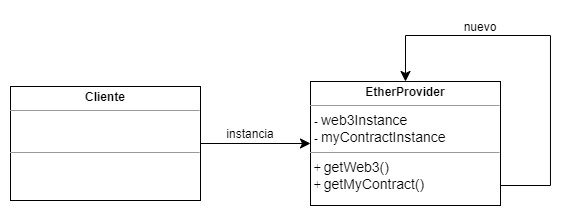
\includegraphics[width=\textwidth]{singleton}
	\caption[Diagrama Singleton]{Diagrama UML de la estructura del Singleton.}
\end{figure}

La implementación de patrón Singleton en el proyecto ofrece ventajas significativas: 

\begin{itemize}
\item \textbf{Eficiencia de recursos}: Solo se crea una instancia, ahorrando recursos y evitando la sobrecarga de establecer múltiples conexiones a la red.

\item \textbf{Consistencia}: Se mantiene una única conexión a lo largo de toda la aplicación, asegurando que todas las operaciones sobre la \textit{blockchain} se manejan de manera consistente.

\item \textbf{Gestión Centralizada}: Facilita la gestión y acceso a la red \textit{blockchain}, ya que los cambios en la conexión se manejan en un único lugar.
\end{itemize}

\subsection{Patrón Módulo}

El Patrón de Módulos es una pieza fundamental en la estructura de diseño y organización del código, permitiendo una clara división y encapsulación de funcionalidades dentro de la aplicación. Este patrón se manifiesta a través de la separación lógica de diferentes áreas de funcionalidad en directorios y archivos específicos, cada uno destinado a manejar distintos aspectos del sistema, facilitando así tanto el desarrollo como el mantenimiento de la aplicación.

Por ejemplo, la aplicación incluye directorios como `Contracts', `components', `Screens' o `AppLogin', cada uno abordando un conjunto específico de responsabilidades dentro de la aplicación:

\begin{itemize}
\item \textbf{Contracts}: Gestiona toda la lógica relacionada con los contratos inteligentes.

\item \textbf{AppLogin}: Maneja la autenticación de usuarios.

\item \textbf{Components}: Contiene elementos de UI reutilizables como botones.

\item \textbf{Screens}: Encapsula los componentes de UI para cada pantalla de la aplicación.
\end{itemize}

Esta modularización asegura que los cambios dentro de un módulo específico puedan realizarse sin afectar a otras partes del sistema. Al mantener cada módulo independiente, se mejora significativamente la legibilidad y la mantenibilidad del código.

\section{Diseño de interfaces}

Antes del desarrollo de la interfaz de la aplicación, se experimentó y depuró un prototipo de la misma.
Las interfaces fueron diseñadas teniendo en cuenta la usabilidad de la aplicación, priorizando un diseño simple que permitiera que la aplicación fuera intuitiva, con una curva de aprendizaje suave.
También se ha considerado que la aplicación sea adaptable a una amplia variedad de pantallas, ya que puede ser utilizada tanto en dispositivos móviles como en tabletas.

El diseño de los prototipos para la aplicación incluye varias pantallas clave: pantalla de inicio de sesión, permitiendo la autenticación de los usuarios (ver imagen \ref{img:prototipoLogin}); la pantalla principal, que actúa como punto de entrada intuitivo (ver imagen \ref{img:prototipoHome}); la pantalla de creación de contratos, donde los usuarios pueden interactuar de manera clara y directa para establecer acuerdos(ver imagen \ref{img:prototipoCrearContrato}); la pantalla de visualización de contratos , diseñada para proporcionar una experiencia fluida al revisar contratos existentes (ver imagen \ref{img:prototipoVerContratos}); la pantalla de información y utilidades, que ofrece recursos y herramientas fácilmente accesibles (ver imagen \ref{img:prototipoInfo}); y la pantalla de estado de cuenta, que muestra de manera clara y concisa la información financiera relevante del usuario (ver imagen \ref{img:prototipoCartera}). 

\begin{figure}[h]
	\label{img:prototipoLogin}
	\centering
	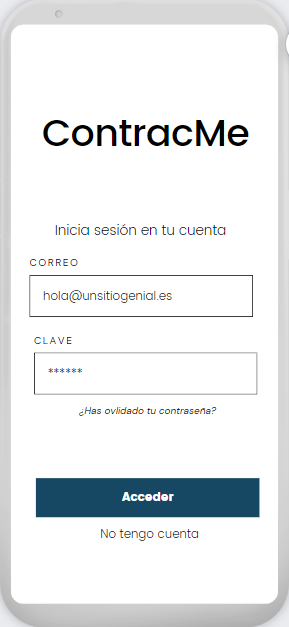
\includegraphics[width=0.55\textwidth]{prototipoLogin}
	\caption[Prototipo pantalla inicio de sesión]{Prototipo pantalla inicio de sesión.}
\end{figure}

\begin{figure}[h]
	\label{img:prototipoHome}
	\centering
	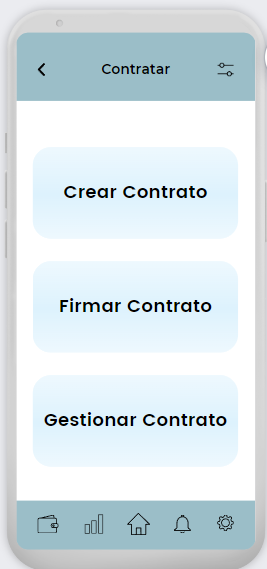
\includegraphics[width=0.55\textwidth]{prototipoHome}
	\caption[Prototipo pantalla principal]{Prototipo pantalla principal.}
\end{figure}

\begin{figure}[h]
	\label{img:prototipoCrearContrato}
	\centering
	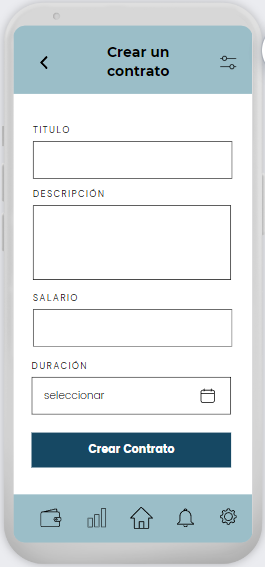
\includegraphics[width=0.55\textwidth]{prototipoCrearContrato}
	\caption[Prototipo pantalla crear contrato]{Prototipo pantalla crear contrato.}
\end{figure}

\begin{figure}[h]
	\label{img:prototipoVerContratos}
	\centering
	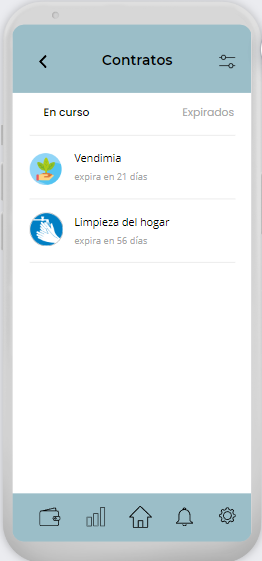
\includegraphics[width=0.55\textwidth]{prototipoVerContratos}
	\caption[Prototipo pantalla ver contratos del usuario]{Prototipo pantalla ver contratos del usuario.}
\end{figure}

\begin{figure}[h]
	\label{img:prototipoInfo}
	\centering
	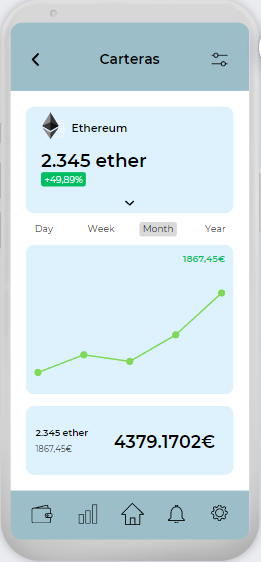
\includegraphics[width=0.55\textwidth]{prototipoInfo}
	\caption[Prototipo pantalla información y utilidades]{Prototipo pantalla información y utilidades.}
\end{figure}

\begin{figure}[h]
	\label{img:prototipoCartera}
	\centering
	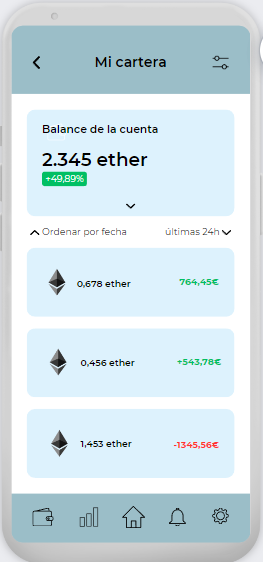
\includegraphics[width=0.55\textwidth]{prototipoCartera}
	\caption[Prototipo pantalla estado cuenta del usuario]{Prototipo pantalla estado cuenta del usuario.}
\end{figure}
